 \documentclass [12pt]{article} 

\usepackage {amsmath}
\usepackage {amsthm}
\usepackage {amssymb}
\usepackage {graphicx} 
\usepackage {float}
\usepackage {multirow}
\usepackage {xcolor}
\usepackage {algorithmic}
\usepackage [ruled,vlined,commentsnumbered,titlenotnumbered]{algorithm2e} \usepackage {array} 
\usepackage {booktabs} 
\usepackage {url} 
\usepackage {parskip} 
\usepackage [margin=1in]{geometry} 
\usepackage [T1]{fontenc} 
\usepackage {cmbright} 
\usepackage [many]{tcolorbox} 
\usepackage [colorlinks = true,
            linkcolor = blue,
            urlcolor  = blue,
            citecolor = blue,
            anchorcolor = blue]{hyperref} 
\usepackage {enumitem} 
\usepackage {xparse} 
\usepackage {verbatim}
\usepackage{listings}
\usepackage{xcolor}
\lstset { %
    language=C++,
    backgroundcolor=\color{black!5}, % set backgroundcolor
    basicstyle=\footnotesize,% basic font setting
}
\newtheorem{theorem}{Theorem}
\newtheorem{remark}{Remark}



\DeclareTColorBox {Solution}{}{breakable, title={Solution}} \DeclareTColorBox {Solution*}{}{breakable, title={Solution (provided)}} \DeclareTColorBox {Instruction}{}{boxrule=0pt, boxsep=0pt, left=0.5em, right=0.5em, top=0.5em, bottom=0.5em, arc=0pt, toprule=1pt, bottomrule=1pt} \DeclareDocumentCommand {\Expecting }{+m}{\textbf {[We are expecting:} #1\textbf {]}} \DeclareDocumentCommand {\Points }{m}{\textbf {(#1 pt.)}} 

\begin {document} 

{\LARGE \textbf {COMP 285 (NC A\&T, Spr `22)}\hfill \textbf {Lecture 5} } 
\vspace {1em} 
\begin {Instruction} 

Adapted From Virginia Williams' lecture notes. Additional credits: J. Su, W. Yang, Gregory Valiant, Mary Wootters, Aviad Rubinstein, Sami Alsheikh.
\end {Instruction} 

\begin{centering}
\section*{Introduce to Recurrences and Master Theorem}
\end{centering}

\section{Introduction to Recurrences}

Recall that divide and conquer algorithms divide up a problem into a number of subproblems that are the smaller instances of the same problem, solve those problems recursively, and combine the solutions to the subproblems into a solution for the original problem. When a subproblem size is small enough, the subproblem is solved in a straightforward manner. In the past lectures we have seen two examples of divide and conquer algorithms: \texttt{MergeSort} and \texttt{Karatsuba}’s algorithm for integer multiplication.

The running time of divide and conquer algorithms can be naturally expressed in terms of the running time of smaller inputs. Today we will show two techniques for solving these recurrences. The first is called the master method to solve these recurrences. This method can only be used when the size of all the subproblems is the same (as was the case in the examples).

\section{Recurrences}
Stated more technically, a divide and conquer algorithm takes an input of size $n$ and does some operations all running in $O(f (n))$ time for some $f$ and runs itself recursively on $k \geq 1$ instances of size $n_1, n_2, \dots n_k$ , where $n_i < n$ for all $i$. To talk about what the runtime of such an algorithm is, we can write a runtime \textbf{recurrence}. Recurrences are functions defined in terms of themselves with smaller arguments, as well as one or more base cases. We can
define a recurrence more formally as follows:

Let $T(n)$ be the worst-case runtime on instances of size $n$. If we have $k$ recursive calls on a given step (of sizes $n_i$) and each step takes time $O(f (n))$, then we can write the runtime as $T(n) \leq c \cdot f (n) + \sum_{i=1}^k T(n_i)$ for some constant $c$, where our base case is $T(c') \leq O(1)$.

Now let’s try finding recurrences for some of the divide and conquer algorithms we have seen.

\subsection{Integer Multiplcation}
Recall the integer multiplication problem, where we are given two $n$-digit integers $x$ and $y$ and output the product of the two numbers. The long multiplication/grade school algorithm runs in $O(n^2)$ time. In lecture 1 we saw two divide and conquer algorithms for solving this problem.
In both of them, we divided each of $x$ and $y$ into two $(n/2)$-digit numbers in the following
way: $x = 10^{\frac{n}{2}} a + b$ and $y = 10^{\frac{n}{2}} c + d$. Then we compute $xy = ac\cdot 10^n + 10^{\frac{n}{2}} (ad + bc) + bd$.

In the first algorithm, which we call \texttt{Mult1}, we simply computed the four products $ac, ad, bc, bd$. Karatsuba found that since we only need the sum of $ad$ and $bc$, we can save one multiplication operation by noting that $ad + bc = (a + b)(c + d) - ac - bd$.

\begin{algorithm}
\caption{Mult1(x,y)}\label{alg:mult1}
\begin{algorithmic}
\STATE Split $x$ and $y$ into $x = 10^{\frac{n}{2}} a + b$ and $y = 10^{\frac{n}{2}} c + d$
\STATE $z_1 = \text{Mult1}(a, c)$
\STATE $z_2 = \text{Mult1}(a, d)$
\STATE $z_3 = \text{Mult1}(b, c)$
\STATE $z_4 = \text{Mult1}(b, d)$
\STATE return $z_1\cdot 10^n + 10^{\frac{n}{2}} (z_2 + z_3) + z_4$
\end{algorithmic}
\end{algorithm}

\begin{algorithm}
\caption{Karatsuba(x,y)}\label{alg:karatsuba}
\begin{algorithmic}
\STATE Split $x$ and $y$ into $x = 10^{\frac{n}{2}} a + b$ and $y = 10^{\frac{n}{2}} c + d$
\STATE $z_1 = \text{Karatsuba}(a, c)$
\STATE $z_2 = \text{Karatsuba}(a, d)$
\STATE $z_3 = \text{Karatsuba}(a+c, c+d)$
\STATE $z_4 = z_3 - z_1 - z_2$
\STATE return $z_1\cdot 10^n + z_4 \cdot 10^{\frac{n}{2}} + z_2$
\end{algorithmic}
\end{algorithm}

We now express the running time of these two algorithms using recurrences. Adding two $n$ digit integers is an $O(n)$ operation, since for each position we add at most three digits: the $i$th digit from each number and possibly a carry from the additions due to the $(i-1)$th digits.

Let $T_1(n)$ and $T_2(n)$ denote the worst-case runtime of Mult1 and Karatsuba, respectively, on inputs of size $n$. Then, the runtime of Mult1 can be written as the recurrence

$$
T_1(n) = 4T_1\left(\frac{n}{2}\right) + O(n)
$$
and Karatsuba's runtime can be written as the recurrence
$$
T_2(n) = 3T_2\left(\frac{n}{2} \right) + O(n)
$$

Note that the constant ``hidden'' in the $O(n)$ term in $T_2$ may be greater than in $T_1$, but for asymptotic analysis of the running time, these constants are not important.

\subsection{MergeSort}
Consider the basic steps for algorithm MergeSort($A$), where $|A| = n$.

\begin{enumerate}
    \item If $|A| = 1$, return $A$.
    \item Split $A$ into $A_1, A_2$ of size $\frac{n}{2}$. 
    \item Run MergeSort($A$) and MergeSort($A_2$).
    \item Merge($A_1, A_2$)
\end{enumerate}

Steps 2 and 4 each take time $O(n)$. In step 3, we are splitting the work up into two subproblems of size $\frac{n}{2}$. Therefore, we get the following recurrence:
$$
T(n) = 2T\left(\frac{n}{2} \right) + O(n)
$$

In the previous lecture, we saw that the running time of MergeSort is O(n\ log n). In this lecture we will show how to derive this using the master method.

\section{The Master Method}

We now introduce a general method, called the \textit{master method}, for solving recurrences where all the subproblems are of the same size. We assume that the input to the master method is a recurrence of the form

$$
T(n) = a \cdot T \left( \frac{n}{b} \right) + O(n^d)
$$

In this recurrence, there are three constants:

\begin{itemize}
    \item $a$ is the number of subproblems that we create from one problem, and must be an integer greater than or equal to $1$.
    \item $b$ is the factor by which the input size shrinks (it must hold that $b > 1$).
    \item $d$ is the exponent of $n$ in the time it takes to generate the subproblems and combine their solutions.
\end{itemize}

There is another constant ``hidden'' in the big-O notation. We will introduce it in the proof and see that it does not affect the result.

In addition, we need to specify the ``base case'' of the recurrence, that is, the runtime when the input gets small enough. For a sufficiently small $n$ (say, when $n = 1$), the worst-case runtime of the algorithm is constant, namely, $T(n) = O(1)$.

We now state the \textit{master theorem}, which is used to solve the recurrences.

\begin{theorem}[Master Theorem]
Let $T(n) = a \cdot T\left(\frac{n}{b}\right) + O(n^d)$ be a recurrence where $a, b > 1$, Then,

\begin{align*}
T(n) &= \begin{cases}
    O(n^d \log n) & \text{if } a = b^d \\
    O(n^d) & \text{if } a < b^d \\
    O(n^{\log_b a}) & \text{if } a > b^d
\end{cases}
\end{align*}
\end{theorem}

\begin{remark}
In some cases, the recurrence may involve subproblems of size $\lceil \frac{n}{b} \rceil, \lfloor \frac{n}{b} \rfloor$ or $nb + 1$. The master theorem holds for these cases as well. However, we do not prove that here.
\end{remark}

Before we turn to the proof of the master theorem, we show how it can be used to solve the recurrences we saw earlier.

\begin{itemize}
    \item Mult1: $T(n) = 4T(\frac{n}{2})+ O(n)$. The parameters are $a = 4, b = 2, d = 1$, so $a > b^d$, hence $T(n) = O(n^{log_2(4)}) = O(n^2)$.
    \item Karatsuba: $T(n) = 3T(\frac{n}{2})+ O(n)$. The parameters are $a = 3, b = 2, d = 1$, so $a > b^d$, hence $T(n) = O(n^{log_2(3)}) = O(n^{1.59})$.
    \item MergeSort: $T(n) = 2T(\frac{n}{2})+ O(n)$. The parameters are $a = 2, b = 2, d = 1$, so $a = b^d$, hence $T(n) = O(n\ log n)$.
    \item Another example: $T(n) = 2T(\frac{n}{2})+ O(n^2)$. The parameters are $a = 2, b = 2, d = 2$, so $a < b^d$, hence $T(n) = O(n^2)$.
\end{itemize}
We see that for integer multiplication, Karatsuba is the clear winner!

\textit{Proof of the Master Theorem} Let $T(n) = a\cdot T(\frac{n}{b})+ O(n^d)$ be the recurrence we solve using the master theorem. For simplicity, we assume that $T(1) = 1$ and that $n$ is a power of $b$. From the definition of big-O, we know that there is a constant $c > 0$ such that for sufficiently large $n$, $T(n) \leq a\cdot T(\frac{n}{b})+ c\cdot n^d$. The proof of the master theorem will use the recursion tree in a similar way to our analysis of the running time of MergeSort.

\begin{figure}[h!]
\centering
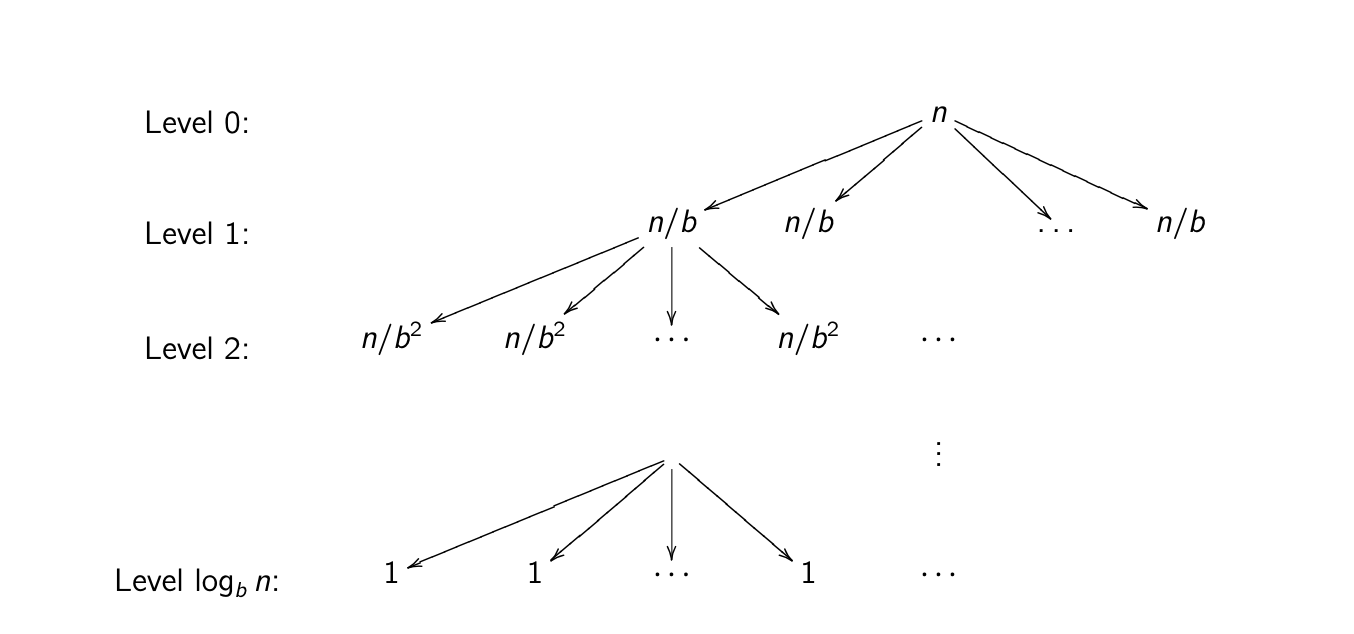
\includegraphics[scale=0.75]{master_theorem_proof.png}
\end{figure}

The recursion tree drawn above has $log_b n + 1$ level. We analyze the amount of work done at each level, and then sum over all levels in order to get the total running time. Consider level $j$. At level $j$, there are $a^j$ subproblems. Each of these subproblems is of size $\frac{n}{b^j}$, and will take time at most $c\left(\frac{n}{b^j}\right)^d$ to solve (this only considers the work done at level $j$ and does not include the time it takes to solve the subsubproblems). We conclude that the total work done at level $j$ is at most $a^j \cdot c\left(\frac{n}{b^j}\right)^d= cn^d\left(\frac{a}{b^d}\right)^j$.

Writing the running time this way shows us where the terms $a$ and $b^d$
come from: $a$ is the branching factor and measures how the number of subproblems grows at each level, and $b^d$ is the shrinkage in the work needed (per subproblem).

Summing over all levels, we get that the total running time is at most $cn^d\Sigma_{j=0}^{\log_b n}\left(\frac{a}{b^d}\right)^j$. We now consider each of the three cases.

\begin{enumerate}
    \item $a = b^d$. In this case, the amount of work done at each level is the same: $cn^d$. Since there are $\log_b n+1$ levels, the total running time is at most $(\log_b n+1)cn^d = O(n^d\ log n)$.
    \item $a < b^d$. In this case, $\frac{a}{b^d} < 1$, hence, $\Sigma^{\log_b n}_{j=0} \left(\frac{a}{b^d}\right)^j \leq \Sigma^{\infty}{j=0} \left(\frac{a}{b^d}\right)^j = \frac{1}{1-\frac{a}{b^d}}= \frac{b^d}{b^d-a}$. Hence, the total running time is $cn^d \cdot \frac{b^d}{b^d-a} = O(n^d)$.

    Intuitively, in this case the shrinkage in the work needed per subproblem is more significant, so the work done in the highest level ``dominates'' the other factors in the running time.
    \item $a > b^d$. In this case, $\Sigma^{\log_b n}_{j=0} \left(\frac{a}{b^d}\right)^j = \frac{\left(\frac{a}{b^d}\right)^{\log_bn+1}-1}{\frac{a}{b^d} -1}$. Since $a, b, c, d$ are constants, we get that the total work done is $O\left(n^d\cdot(\frac{a}{b^d})^{\log_b n}\right) = O\left(n^d\cdot \frac{a^{\log_b n}}{b^{d \log_b n}}\right) = O\left(n^d \cdot \frac{n^{\log_b a }}{n^d}\right)=O\left(n^{\log_b a}\right)$.

    Intuitively, here the branching factor is more significant, so the total work done at each level increases, and the leaves of the tree ``dominate''.
\end{enumerate}

We conclude with a more general version of the master theorem.

\begin{theorem}[Master Theorem - more general version]
Let $T(n) = a \cdot T(\frac{n}{n}) + f(n)$ be a recurrence where $a \geq 1, b > 1$. Then, 
    \begin{itemize}
        \item If $f(n) = O(n^{\log_n(a) - \epsilon})$ for some constant $\epsilon > 0, T(n) = \Theta(n^{\log_b (a)})$.
        \item If $f(n) = \Theta(n^{\log_b(a)})$, $T(n) = \Theta(n^{\log_b (a)} \log n)$.
        \item If $f(n) = \Omega(n^{\log_n(a) + \epsilon})$ for some constant $\epsilon > 0$ and if $af(n/b) \leq cf(n)$ for some $c < 1$ and all sufficiently large $n$, then $T(n) = \Theta(f(n))$.
    \end{itemize}
\end{theorem}
\end{document}